% Chapter 4

\chapter{Travaux et apports} % 4th chapter title

\label{Chapter4} % For referencing the chapter elsewhere, use \ref{Chapter4} 


%----------------------------------------------------------------------------------------


\section{Les missions du poste}

\begin{itemize}
    \item L'état de l'art de la partie précédente fait partie des missions.
    \item Modélisation
    \item Simulation
\end{itemize}

Nous souhaitons étudier le comportement mécanique d'un floe après collision avec un autre floe. Les étapes de travail envisagées sont les suivantes:
\begin{enumerate}
    \item Ecire les systèmes differentiels pour les deux floes juste après le choc: pour l' instant on peut considérer que l'un des floes est immobile (celà revient au même si l'on exprimes les vitesses dans un repère lié à ce floe).
    \item On exprime l'EDO vérifiée par les solutions, c'est à dire $q$ pour le premier floes, et $p$ pour le second.
    \item On pourra ensuite simuler ces EDP limites et trouver les valeurs de $p$ et $q$. Autrement dit, on connait la position de chaque point du réseau au temps final.
    \item Si on connait $p$ et/ou $q$, on connait la condition de Dirichlet sur le floe concerné, et on peut ainsi exprimer le déplacement et la possible fracture du floe. 
\end{enumerate}




\section{Présentation des résultats obtenus}



\subsection{Modélisation générale du contact entre deux floes de glace}

Les floes de glace $\Omega_k$ et $\Omega_l$ sont modélisés par des systèmes masse-ressort (à grande raideur). Pour l'instant, nous considérons une moélisation simplifiée qui assimile un floe à un système de (trois) masses reliés par des ressorts (de constante de raideur $k$), et par des dispositifs visqueux de constante $\mu$.
Nous désignerons par $n+1$ le nombre total de noeuds du floe $\Omega_k$, chaque noeud ayant pour masse $m$. De facon similaire, on définit les constantes $k'$, $\mu'$, $n'+1$, $m'+1$ pour le floe $\Omega_l$. Les positions des noeds de $\Omega_k$ seront noté $(q_i)_{0\leq i\leq n}$, tandis que ceux de $\Omega_l$ seront notés $(p_i)_{0 \leq i\leq n'}$ (voir \cref{fig:contactmanuel}). 

\begin{figure}[!h]
    \centering
    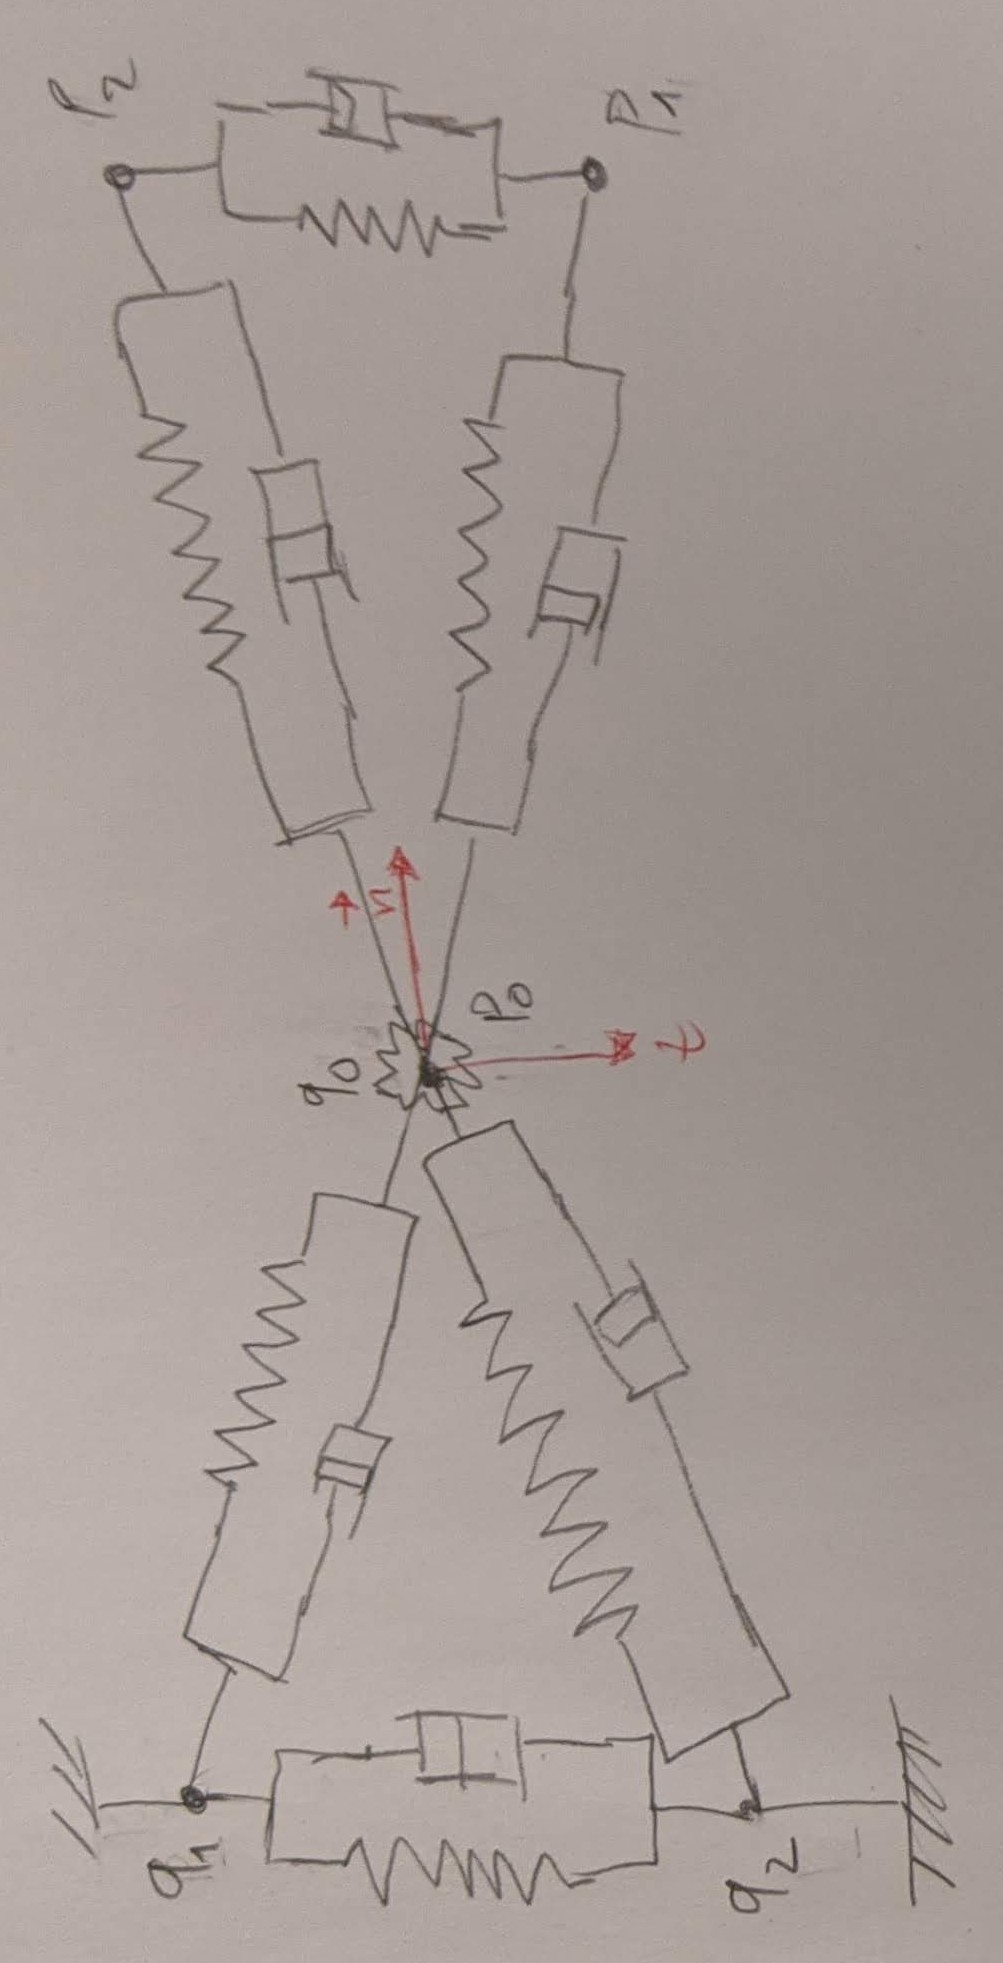
\includegraphics[width=0.3\textwidth, angle=-90]{ContactManuel.jpg}
    \caption{Contact entre deux floes aux points $p_0 = q_0$.}
    \label{fig:contactmanuel}
\end{figure}

\noindent On définit la matrice de contact $C$...(voir these Dimitri), et $L_{0j}$.. et $u_{0j}$ ..

\noindent Comme présenté dans les travaux \parencite[p.186]{balasoiu2020halthesis}, le système différentiel qui modélise la percussion s’écrit comme le couplage de deux sous-systèmes. Le premier, dit système intérieur (SI), est à évolution rapide et modélise la propagation des ondes élastiques dans le système masse-ressort. Ici, nous dérivons facilement et réutilisont le SI comme présenté par \citeauthor{balasoiu2020halthesis}. Le second, dit système extérieur (SE), est à évolution lente et modélise la pénétration de l’objet solide dans le système masse-ressorts. Pour dériver le SE sur le floe $\Omega_k$, nous écrivons l'équation de Newton-Euler linéaire\footnote{La rotation du point matériel $q_0$ n'est pas prise en compte ici, d'où l'abscence de l'équation de Newton-Euler angulaire.} au point de contact $q_0$:
\begin{align}  \label{eq:SE}
m \ddot{\bvec{q}}_0 = \bvec{F}_0 + \bvec{F}^c_0 \,,
\end{align}
où 
\begin{align}  \label{eq:F0}
    \bvec{F}_0 = \sum_{j=0}^{n}C_{0j} \left[  \underbrace{k \left( \Vert \bvec{q}_j - \bvec{q}_0 \Vert - L_{0j} \right) \bvec{u}_{0j}}_{\text{Force de rappel}} - \underbrace{\mu \left\langle \bvec{\dot{q}}_j - \bvec{\dot{q}}_0\,, \bvec{u}_{0j}  \right\rangle  \bvec{u}_{0j}}_{\text{Force de dissipation}}  \right] \,,
\end{align}
représente la somme des forces de reaction et de disssipation exercées par le ressort et le dispositif visqueux sur le noeud $q_0$ ; et $\bvec{F}^c_0(t)$ la force de contact durant la collison entre les deux particules. En supposnat qu'il existe un repère de contact $\mathcal{R}^c = \{ q_0, \bvec{n}, \bvec{t} \}$ associé au floe $\Omega_k$ (voir \cref{fig:contactmanuel}), on peut écrire, pour $(\lambda, \beta) \in \Rdeux$ :
\begin{align}  \label{eq:F0c}
    \bvec{F}_0^c = \lambda \bvec{n} + \beta \bvec{t} \,.
\end{align}
Le système intérieur (SE) s'obtient facilement en combinant les équations \cref{eq:SE,eq:F0,eq:F0c}. Le système intérieur (SI) s'obtient lui (pour les autres noeuds du réseau) en y supprimant la force de contact. On obtient au final:
\begin{align} \tag{$E$} \label{eq:e}
\begin{dcases}
    m \ddot{\bvec{q}}_0 = \bvec{F}_0 + \bvec{F}^c_0  \,, &\qquad \text{(SE)} \\
    m \ddot{\bvec{q}}_i = \bvec{F}_i   \,, \quad \quad \quad \forall 1 \leq i \leq n \,. &\qquad \text{(SI)}
\end{dcases}
\end{align}
En ce qui concerne le floe $\Omega_l$, nous procédons de facons similaire et appliqons la 3ème loi de Newton (action-réaction) pour obtenir le système:
\begin{align} \tag{$E'$} \label{eq:eprime}
\begin{dcases}
    m' \ddot{\bvec{p}}_0 = \bvec{F}^{'}_0 - \bvec{F}^c_0  \,, &\qquad \text{(SE)} \\
    m' \ddot{\bvec{p}}_i = \bvec{F}^{'}_i   \,, \quad \quad \quad \forall 1 \leq i \leq n' \,, &\qquad \text{(SI)}
\end{dcases}
\end{align}
où $(\bvec{F}^{'}_i)_{0 \leq i \leq n'}$ sont définis de facon similaire à $\bvec{F}_0$ (voir \cref{eq:F0}).

Ensuite, il nous faut introduire des conditions portant sur la conservation de l'énergie, et la condition de non-interpénétration de Signorini\dots



\subsection{Modélisation et simulation 1D}



\subsubsection{Collision parfaitement inélastique avec un floe immobile à l'instant initial}

Nous effectuons ici une modélisation 1D de notre problème. Un floe est modélisé par un système masse-ressort de deux nœuds. Le floe 1 est immobilisé face au mur, et le floe 2 approche à la vitesse $\bvec{v}_0$. On identifie les nœuds $q_0$ et $p_0$ de la section précédente à leur masses respectives $m$ et $m'$ (voir \cref{fig:contact1d}).
\begin{figure}[!h]
    \centering
    \frame{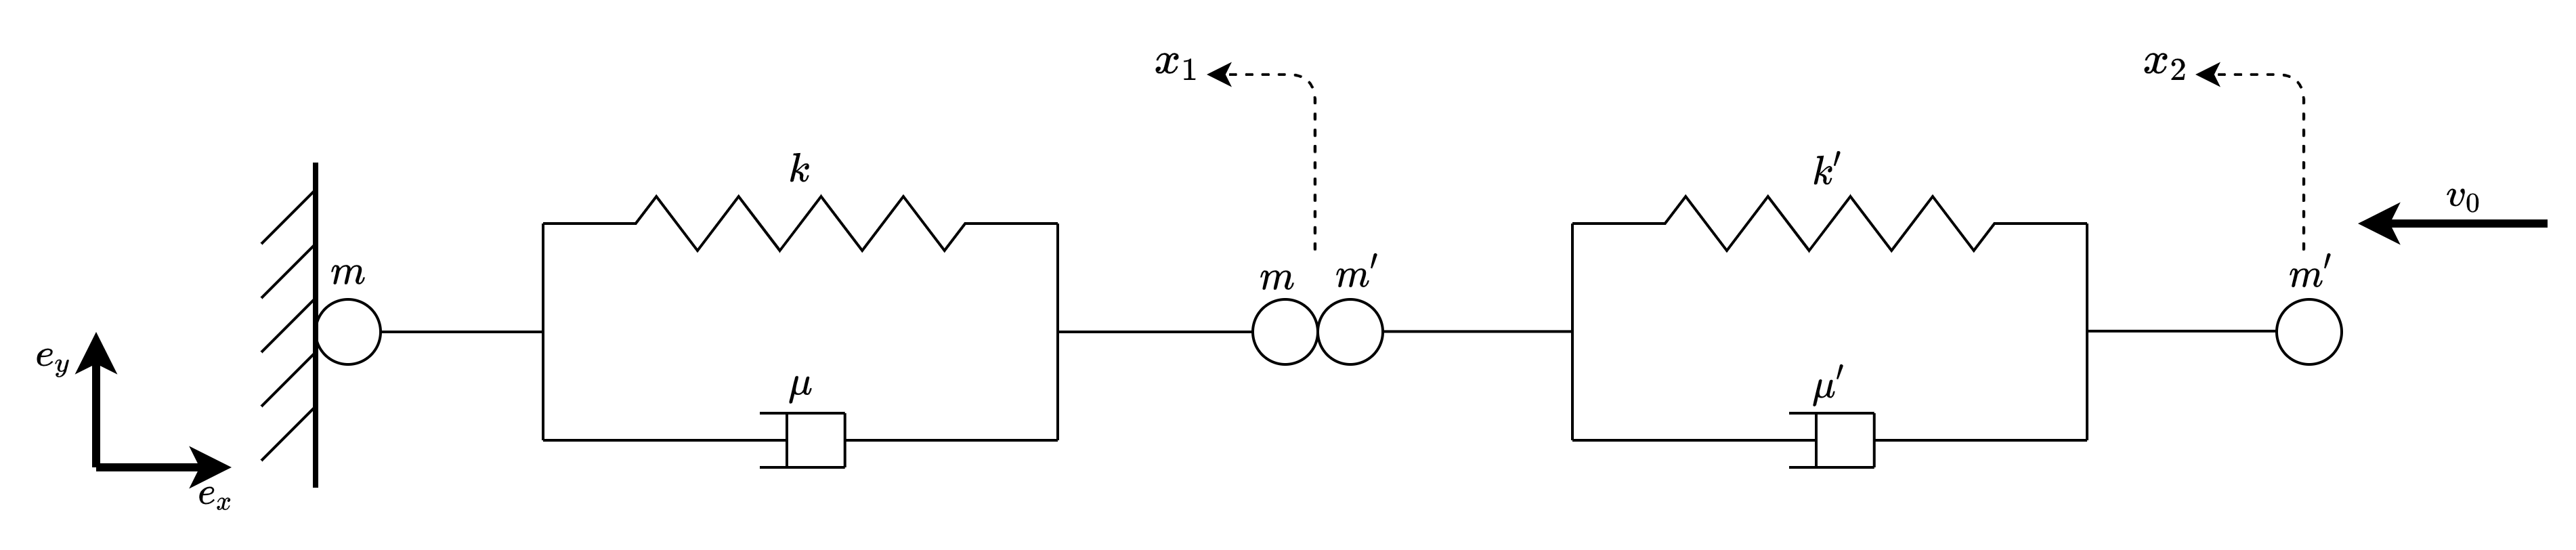
\includegraphics[width=0.8\textwidth]{Percussion1D-Systeme}}
    \caption{Contact 1D parfaitement inélastique entre deux floes. Le floe percuté étant immobile et coincé au mur avant le choc.}
    \label{fig:contact1d}
\end{figure}

\noindent On suppose que durant la dynamique non régulière, les masses $m$ et $m'$ en contact forment une seule masse
$m+m'$ dont
le déplacement est donné par la variable $x_1(t)$. Le déplacement de la masse $m'$ à l'autre bout du floe percuteur est nommé
$x_2(t)$. La masse $m$ qui est fixée au mur ne sera pas étudiée ici. Nous faisons à présent le bilan des forces qui
s'exercent ces
deux masses.
\begin{figure}[!h]
     \begin{subfigure}[b]{0.4\textwidth}
         \centering
         \frame{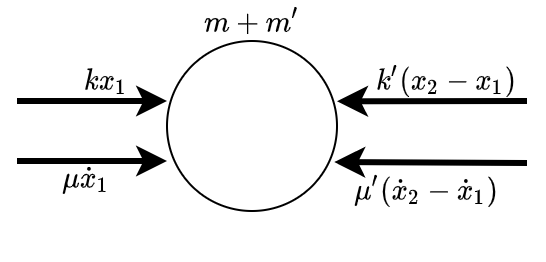
\includegraphics[width=\textwidth]{Percussion1D-Masse1}}
         \caption{Sur $m+m'$.}
         \label{fig:bilan11}
     \end{subfigure}
%     \hfill
     \begin{subfigure}[b]{0.3\textwidth}
         \centering
         \frame{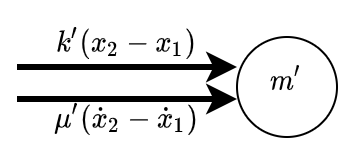
\includegraphics[width=\textwidth]{Percussion1D-Masse2}}
         \caption{Sur $m'$.}
         \label{fig:bilan12}
     \end{subfigure}
        \caption{Bilan des forces appliquée sur les noeuds du système. Les valeurs indiquées sont les intensitées
            (positives) des forces durant une phase imaginée de compression des ressorts ($\bvec{v}_0 <0$ et donc
            $x_1 <0$). Pour obtenir l'intesité de la force de rappel du ressort $k'$, on peut imaginer $x_1$ imobile
            (on aura $x_2 < 0$, d'où $x_1 - x_2 > 0$).}
        \label{fig:bilan}
\end{figure}

\noindent En orientant convenablement le système (voir \cref{fig:contact1d}), on applique la loi de Newton-Euler linéaire
pour obtenir le système suivant et ses conditions initiales \footnote{J'ai des doutes sur cette condition
initiale. La vitesse initiale de $x_1$ est-elle vraiment nulle?}:
\begin{align}
    \begin{dcases}
    (m+m')\ddot x_1 = -kx_1 - \mu \dot x_1 + k'(x_2 - x_1) + \mu'(\dot x_2 - \dot x_1) \\
        m' \ddot x_2 =  -k'(x_2 - x_1) - \mu'(\dot x_2 - \dot x_1) \\
    \end{dcases}
\end{align}
À l'instant initial $t_0$, on a le système suivant
\begin{align} \label{eq:percussion1d}
    \begin{dcases}
    (x_1(t_0), x_2(t_0)) = (0,0) \\
    (\dot x_1(t_0), \dot x_2(t_0)) = (0,-v_0)
    \end{dcases}
\end{align}
En posant $X = (x_1, x_2)^T \in \mathbb{R}^2$, l' \cref{eq:percussion1d} devient
\begin{align}
    \underbrace{\mymat{m+m'}{0}{0}{m'}}_{A} \myvec{\ddot{x}_1}{\ddot{x}_2} = \underbrace{\mymat{-\mu -
    \mu^\prime}{\mu'}{\mu'}{-\mu'}}_{B}
    \myvec{\dot{x}_1}{\dot{x}_2} + \underbrace{\mymat{-k-k'}{k'}{k'}{-k'}}_{C} \myvec{x_1}{x_2} \,.
\end{align}
Puisque $m, m'\neq 0$, la matrice $A$ est inversible et on obtient au final le problème de Cauchy suivant:

\begin{align} \label{eq:percussion1d2}
    \begin{dcases}
        \ddot{X}(t) = B' \dot{X}(t) + C'X(t) \,, \\
        (X(t_0), \dot X (t_0)) = \left( \myvec{0}{0}, \myvec{0}{-v_0} \right) \,,
    \end{dcases}
\end{align}
avec $B' = A^{-1}B$ et $C' = A^{-1}C$.

\noindent Il s'agit la d'un système d'EDO du deuxième ordre à coefficients constants. Transformons le en un système du
premier ordre pour
une
résolution plus aisée. On pose donc $Y= (X, \dot X)^T = (x_1, x_2, \dot{x}_1, \dot{x}_2)^T \in \mathbb{R}^4$ et le
système
\ref{eq:percussion1d2}
devient
\begin{align} \label{eq:systeme1d}
    \begin{dcases}
        \dot{Y}(t)= E Y(t) \\
        Y_0 = Y(t_0) = (0,0,0,-v_0)^T
    \end{dcases}
\end{align}
avec la matrice par blocs \[ E = \mymat{0}{I_2}{C'}{B'} \,, \] où $I_2$ désigne la matrice identité de
$\mathbb{R}^{2\times2}$.

\noindent Avec $t_0= 0$, la solution de ce système d'EDO du premier ordre à coefficients constants est unique et est donnée par
\begin{align}
    Y(t) = \exp(tE)Y_0
\end{align}

La résolution numérique du système passe par le calcul de l'exponentielle de la matrice $E \in  \mathbb{R}^4$ (VOIR figure ci-bas et NOTEBBOK ) \ldots
\begin{figure}[!h]
    \centering
    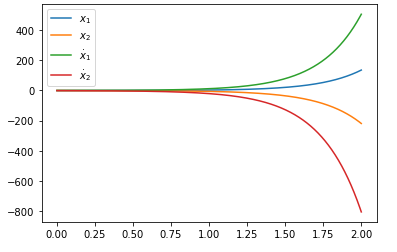
\includegraphics[width=0.4\textwidth]{SimuPercussion1D.png}
    \caption{Simulation de la percussion 1D entre deux floes avec $m=1$, $m'=1$, $k=16$, $k'=5$, $\mu=6$,
        $\mu'=2$, $v_0=-1.0$, $t_{max}=32$. On observe effectivement le ralentissement du système et une convergence
        vers l'état d'équilibre $Y_{eq}= (0,0,0,0)$.}
    \label{fig:simucontact1d}
\end{figure}

\noindent Pour certaines valeurs (specifiquement de $\mu$ et $\mu'$), on constate que le système converge vers son état d'équilibre attendu $Y_{eq} = (0,0,0,0)$. Il nous reste dans cette section:
\begin{enumerate}
    \item Calculer analytiquement et numériquement tous les état d'équilibres $Y_{eq} \in \ker(E)$; distinguer les états stables des autres.
    \item Calculer analytiquement l'exponentielle de la matrice $E$, et donner l'expression de la solution; déduire la condition sur les parametres pour que le système converge vers l'état d'équilibre voulu.
\end{enumerate} 




\subsubsection{Collision parfaitement inélastique sans présence du mur}

Contrairement au cas étudié dans la section précédente, le mur est supprimé dans cette section. On obtient donc une troisième varaible $x_3$ décrivant le comportement du noed qui était rattaché au mur. La schéma régissant ce système est donnée à la \cref{fig:contact1d2}. Le bilan des forces appliquées aux noeuds est présenté à la \cref{fig:bilan2}.

\begin{figure}[!h]
    \centering
    \frame{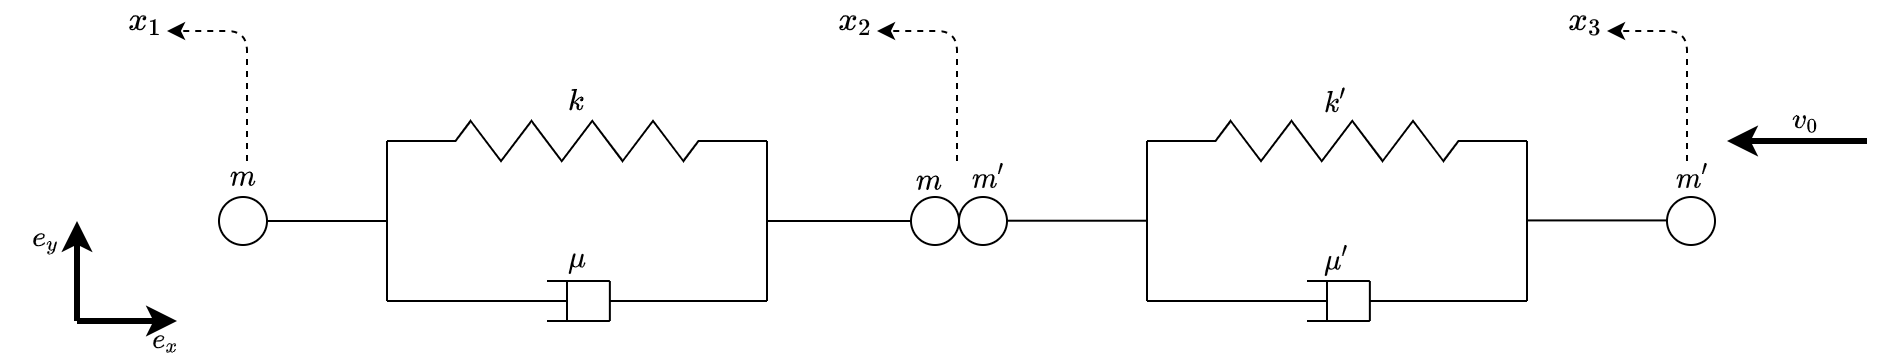
\includegraphics[width=0.8\textwidth]{Percussion1D-Systeme-2}}
    \caption{Contact 1D parfaitement inélastique entre deux floes. Le floe percuté étant immobile mais non coincé au mur avant le choc. On représnte également les variables $x_1$, $x_2$, et $x_3$ décrivant les movements de chaque noeud.}
    \label{fig:contact1d2}
\end{figure}

\begin{figure}[!h]
    \begin{subfigure}[b]{0.25\textwidth}
        \centering
        \frame{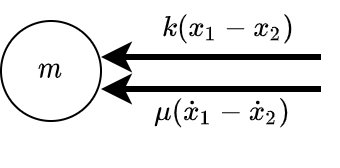
\includegraphics[width=\textwidth]{Percussion1D2-Masse1.png}}
        \caption{Sur $m$.}
        \label{fig:bilan12}
    \end{subfigure}
%     \hfill
    \begin{subfigure}[b]{0.31\textwidth}
        \centering
        \frame{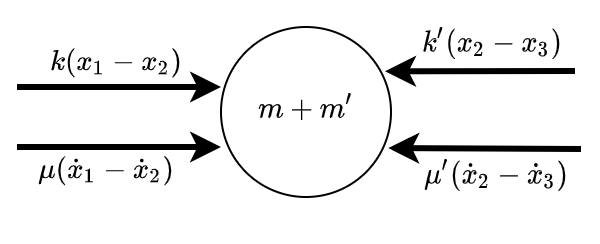
\includegraphics[width=\textwidth]{Percussion1D2-Masse2}}
        \caption{Sur $m+m'$.}
        \label{fig:bilan22}
    \end{subfigure}
%     \hfill
    \begin{subfigure}[b]{0.23\textwidth}
        \centering
        \frame{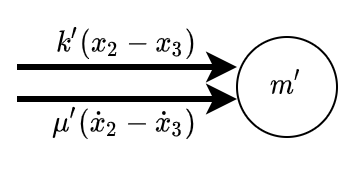
\includegraphics[width=\textwidth]{Percussion1D2-Masse3}}
        \caption{Sur $m'$.}
        \label{fig:bilan32}
    \end{subfigure}
       \caption{Bilan des forces appliquée sur les noeuds du système. On procède de facon similaire à \cref{fig:bilan} pour obtenir les sens et les intensités de ces forces.}
       \label{fig:bilan2}
\end{figure}

\noindent Comme précédement, nous appliqons les lois de Newton pour obtenir:
\begin{align}
    \begin{dcases}
    m\ddot x_1 = -k(x_1 - x_2) - \mu (\dot x_1 - \dot x_2) \,, \\
    (m+m')\ddot x_2 = k(x_1 - x_2) + \mu (\dot x_1 - \dot x_2) - k'(x_2 - x_3) - \mu'(\dot x_2 - \dot x_3) \,, \\
        m' \ddot x_3 =  k'(x_2 - x_3) + \mu'(\dot x_2 - \dot x_3) \,. \\
    \end{dcases}
\end{align}
Sous forme matricielle, on a
\begin{align}
    \underbrace{\mybigmat{m}{0}{0}{0}{m+m'}{0}{0}{0}{m'}}_{A} \mybigvec{\ddot{x}_1}{\ddot{x}_2}{\ddot{x}_3} =  
    \underbrace{\mybigmat{-k}{k}{0}{k}{-k-k'}{k}{0}{k'}{-k'}}_{B} \mybigvec{x_1}{x_2}{x_3} + 
    \underbrace{\mybigmat{-\mu}{\mu}{0}{\mu}{-\mu-\mu'}{\mu'}{0}{\mu'}{-\mu'}}_{C} \mybigvec{\dot{x}_1}{\dot{x}_2}{\dot{x}_3} \,.
\end{align}
Puisque $m, m'\neq 0$, la matrice $A$ est inversible. En posant $X = (x_1, x_2, x_3)^T \in \mathbb{R}^3$, le système d'EDO revient à l' \cref{eq:percussion1d22} suivante:
\begin{align} \label{eq:percussion1d22}
        \ddot{X}(t) = B' X(t) + C'\dot{X}(t) \,, 
\end{align}
où $B' = A^{-1}B$ et $C' = A^{-1}C$. On pose ensuite $Y= (X, \dot X)^T \in \mathbb{R}^6$ et le système \cref{eq:percussion1d22} devient 
\begin{align} \label{eq:systeme1d2}
        \dot{Y}(t)= E Y(t)
\end{align}
avec $$ E = \mymat{0}{I_3}{B'}{C'} \,.$$.


Remarquons qu'en enlevant le mur à gauche du domaine (voir \cref{fig:contact1d}), le système est devenu isolé. Nous pouvons donc appliquer la conservation de la quantité de mouvement pour identifier la vitesse de l'ensemble $m+m'$ après collision et fixation de la masse $m'$ (à vitesse $\bvec{v}_0$) sur la masse $m$ (de vitesse nulle). Pour simplifier les calculs, nous considérons les floes comme des solides rigides. La vitesse de l'ensemble juste après collision est notée $v_f$, et la quantité de mouvement avant et après choc sont notées $P_{\text{avant}}$ et $P_{\text{après}}$. On a:
\begin{align*}
    & \quad P_{\text{avant}} = P_{\text{après}} \\
    \Rightarrow & \quad 2m'\bvec{v}_0 = (2m + 2m') \bvec{v}_f \\
    \Rightarrow & \quad \bvec{v}_f = \frac{m'}{m+m'}\bvec{v}_0
\end{align*} 

\noindent On introduit ces conditions initiales dans l'\cref{eq:systeme1d2} pour obtenir le système de Cauchy ci-bas. Le résulat de la simulation est présenté à la figure \cref{fig:simucontact1d2}. 
\begin{align} \label{eq:systeme1d3}
    \begin{dcases}
        \dot{Y}(t)= E Y(t) \,, \\
        Y(t_0) = Y_0 = -v_f(0,0,0,1,1,1) \,.        
    \end{dcases}
\end{align}

\begin{figure}[!h]
    \centering
    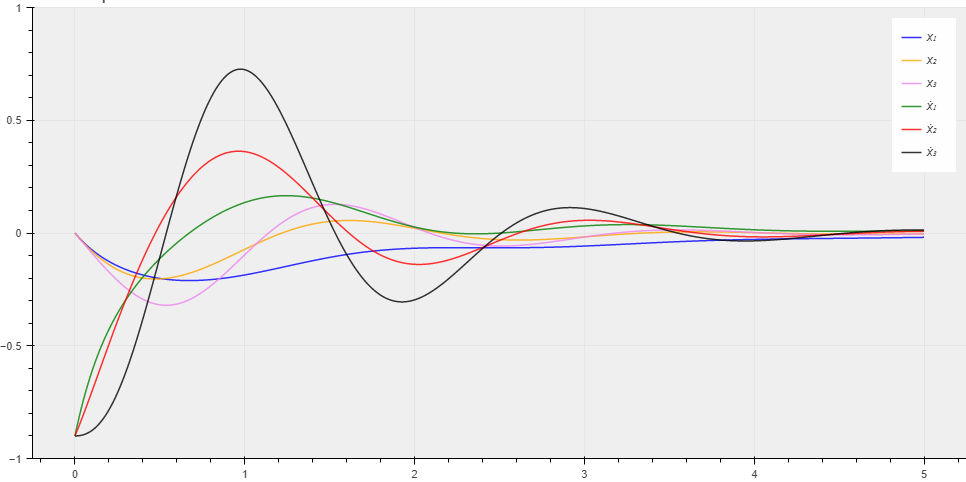
\includegraphics[width=0.6\textwidth]{SimuPercussion1D2.png}
    \caption{Simulation de la percussion 1D entre deux floes (sans présence du mur) avec $m=1$, $m'=1$, $k=3$, $k'=22$, $\mu=6$,$\mu'=2$, $v_0=-1.8$, $t_{max}=5$. On observe effectivement le ralentissement du système et une convergence vers l'état d'équilibre $Y_{eq}= (0,0,0,0,0,0)$.} 
    \label{fig:simucontact1d2}
\end{figure}









\section{Les apports du stage}

%\begin{itemize}
%    \item L' utilisation de TIKZ
%\end{itemize}